%!TEX encoding = UTF-8 Unicode
\documentclass{lecturenotes}

\renewcommand{\vecka}{4}
\newcommand{\veckotema}{Datastrukturer}

%!TEX encoding = UTF-8 Unicode
\setbeamertemplate{footline}[frame number]
\title[Föreläsningsanteckningar EDAA45, 2016]{EDAA45 Programmering, grundkurs}
\subtitle{Läsvecka \vecka: \veckotema}
\author{Björn Regnell}
\institute{Datavetenskap, LTH}
\date{Lp1-2, HT 2016}








 
\begin{document}

\frame{\titlepage}
\setnextsection{\vecka}
\section[Vecka \vecka: \veckotema]{\veckotema}
\frame{\tableofcontents}

\ifkompendium\else
\begin{Slide}{Denna vecka: Datastrukturer och IDE}
\begin{itemize}
\item Datastrukturer med tupler, klasser och färdiga samlingar
\begin{itemize}
\item Mer om klasser senare: 
\begin{itemize}
\item w06 Klasser \item w07 Arv \item w09 Typparametrar
\end{itemize}

\item Mer om samlingar senare: 
\begin{itemize}
\item w05 Sekvensalgoritmer \item w09 Matriser \item w10 Sökning, Sortering
\end{itemize}
\end{itemize}

\item Övning \texttt{data}: prova tupler, klasser och samlingsmetoder

\item Laboration \texttt{pirates}: prata som pirater och prova IDE

\item Börja använda en integrerad utvecklingsmiljö (IDE),\\labbförberedelse bl.a.: läs appendix D och få igång en IDE

\end{itemize}
\end{Slide}
\fi

%!TEX encoding = UTF-8 Unicode
%!TEX root = ../lect-week04.tex

\ifkompendium\else

\begin{Slide}{Denna vecka: Fatta datastrukturer}
\begin{itemize}
\item Läs teori
\item Gör övning \code{data}
\item Gör lab \code{???}
\end{itemize}
\end{Slide}

\fi

%%%

\begin{Slide}{Olika sätt att skapa datastrukturer}
\begin{itemize}
\item Tupler
  \begin{itemize}
  \item samla $n$ st datavärden i element \Emph{\code{_1}}, \Emph{\code{_2}}, ...  \code{_}$n$
  \item elementen kan vara av \Alert{olika} typ
  \end{itemize}
\item Klasser   
  \begin{itemize}
  \item samlar data i \Emph{attribut} med (väl valda!) namn
  \item attributen kan vara av \Alert{olika} typ
  \item definierar även metoder som använder attributen (operationer på data)
  \end{itemize}

\item Samlingar 
  \begin{itemize}
  \item speciella klasser som samlar data i element av \Alert{samma} typ
  \item finns ofta \emph{många} färdiga \Emph{bra-att-ha-metoder} 
  \end{itemize}
\end{itemize}
\end{Slide}

\ifkompendium\else

\begin{Slide}{Vad är en tupel?}
\code{("hej", 42, math.Pi)} är en 3-tupel med typ: \code{(String, Int, Double)}
\end{Slide}

\fi


\begin{Slide}{Hierarki av samlingar i scala.collection}
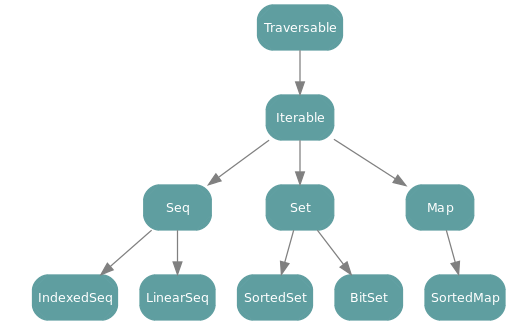
\includegraphics[width=1.0\textwidth]{../img/collection/collection-traits}
\end{Slide}

\ifkompendium
\noindent Läs mer om Scalas samlingar här: \\ 
\url{http://docs.scala-lang.org/overviews/collections/overview}
\else\fi

\ifkompendium\else

\begin{Slide}{scala.collection.immutable}
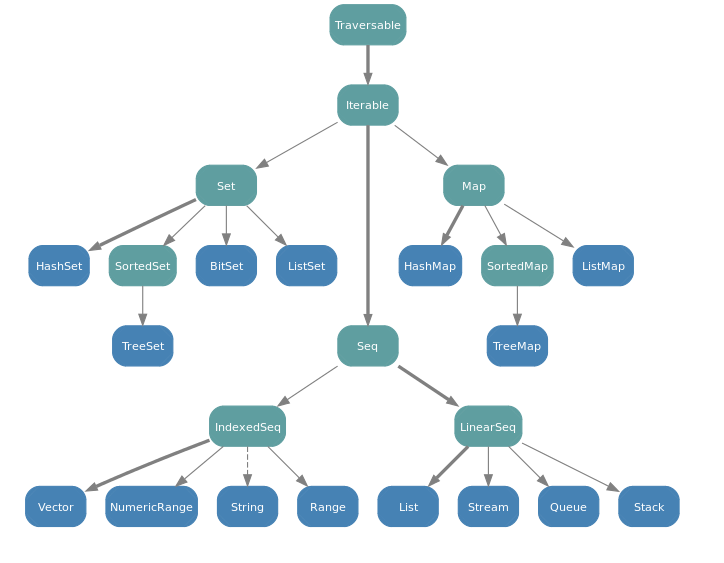
\includegraphics[width=0.82\textwidth]{../img/collection/collection-immutable}
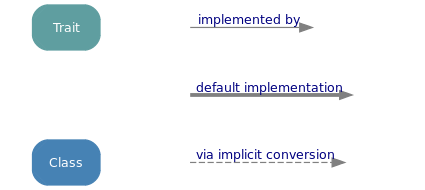
\includegraphics[width=0.33\textwidth]{../img/collection/collection-legend}
\end{Slide}

\begin{Slide}{scala.collection.mutable}
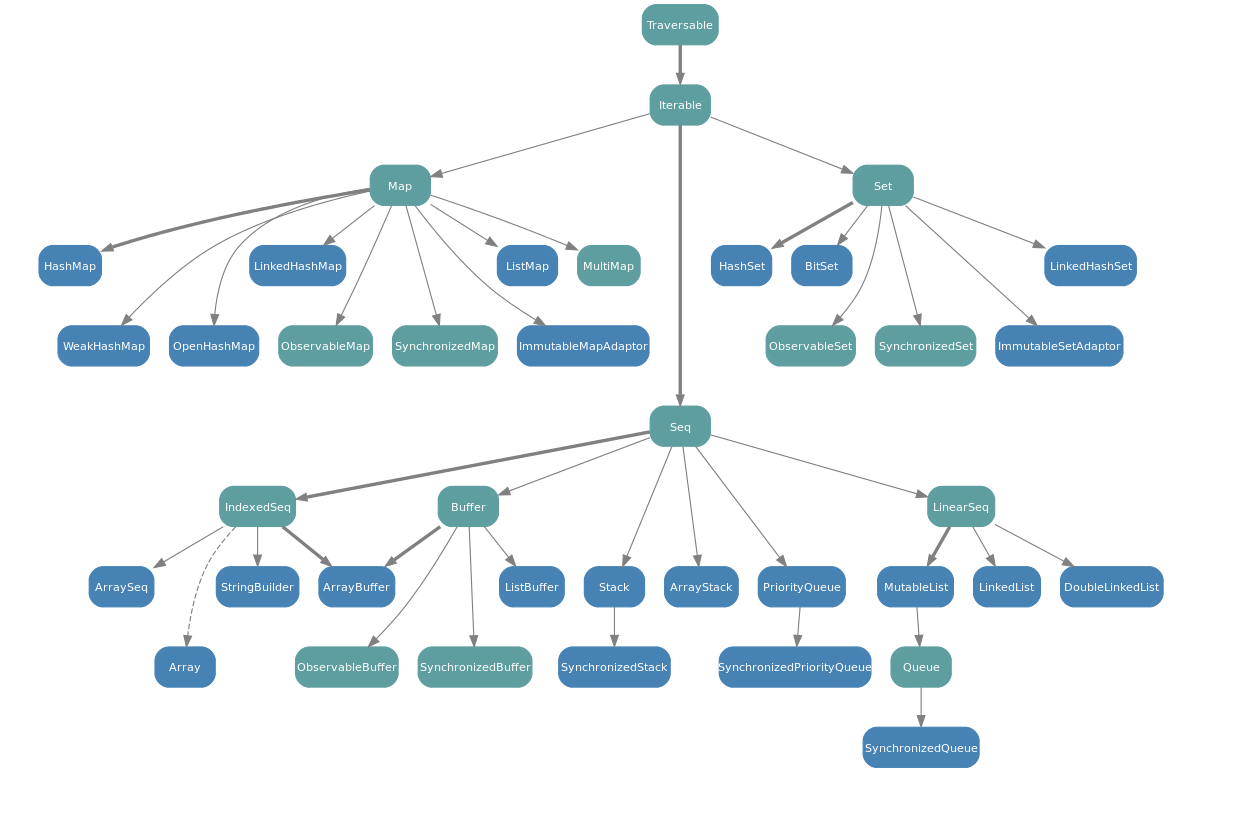
\includegraphics[width=1.05\textwidth]{../img/collection/collection-mutable}
\end{Slide}
\fi


% ??? Berätta om javafx.util.pair
% http://stackoverflow.com/questions/521171/a-java-collection-of-value-pairs-tuples




%!TEX encoding = UTF-8 Unicode
%!TEX root = ../lect-week04.tex

\ifkompendium\else

\Subsection{Tupler}

\begin{Slide}{Vad är en tupel?}\SlideFontSmall

\begin{itemize}
\item En tupel samlar $n$ st objekt i en enkel struktur, med koncis syntax.
  \item Elementen kan vara av \Alert{olika} typ.

\item 
\code{("hej", 42, math.Pi)} är en \Emph{3-tupel} av typen: \code{(String, Int, Double)}

\item Du kan komma åt det enskilda elementen med \Emph{\code{_1}}, \Emph{\code{_2}}, ...  \code{_}$n$

\begin{REPL}
scala> val t = ("hej", 42, math.Pi)
t: (String, Int, Double) = (hej,42,3.141592653589793)

scala> t._1
res0: String = hej

scala> t._2
res1: Int = 42
\end{REPL}

\item Tupler är praktiska när man inte vill ta det lite större arbetet att skapa en egen klass.
(Men med klasser kan man göra mycket mer än med tupler.)

\item I Scala kan du skapa tupler upp till en storlek av 22 element. 
\\ (Behöver du fler element, använd i stället en samling, t.ex. \code{Vector}.)

\end{itemize}

\end{Slide}




\begin{Slide}{Tupler som parametrar och returvärde.}\SlideFontSmall

\begin{itemize}

\item Tupler är smidiga när man på ett enkelt och typsäkert sätt vill låta en funktion \Emph{returnera mer än ett värde}.

\begin{REPL}
scala> def längd(p: (Double, Double)) = math.hypot(p._1, p._2)

scala> def vinkel(p: (Double, Double)) = math.atan2(p._1, p._2) 

scala> def polär(p: (Double, Double)) = (längd(p), vinkel(p))

scala> polär((3,4))
res2: (Double, Double) = (5.0,0.6435011087932844)

\end{REPL}
\vspace{0.5em}
\item Om typerna passar kan man skippa dubbla parenteser vid \Emph{ensamt tupel-argument}:
\begin{REPL}
scala> polär(3,4)
res3: (Double, Double) = (5.0,0.6435011087932844)
\end{REPL}
\item[] {\SlideFontTiny\href{https://sv.wikipedia.org/wiki/Pol\%C3\%A4ra_koordinater}{https://sv.wikipedia.org/wiki/Polära\_koordinater}}


\end{itemize}
\end{Slide}

\begin{Slide}{Ett smidigt sätt att skapa 2-tupler med metoden \texttt{->}}
Det finns en metod vid namn \code{->} som kan användas på objekt av \Alert{godtycklig} typ för att \Emph{skapa par}:

\vspace{0.8em}
\begin{REPL}
scala> ("Ålder", 42)
res0: (String, Int) = (Ålder,42)

scala> "Ålder".->(42)
res1: (String, Int) = (Ålder,42)

scala> "Ålder" -> 42
res2: (String, Int) = (Ålder,42)

scala> Vector("Ålder" -> 42, "Längd" -> 178, "Vikt" -> 65) 
res3: scala.collection.immutable.Vector[(String, Int)] = 
        Vector((Ålder,42), (Längd,178), (Vikt, 65))


\end{REPL}



\end{Slide}


\fi



% ??? Berätta om javafx.util.pair
% http://stackoverflow.com/questions/521171/a-java-collection-of-value-pairs-tuples




%!TEX encoding = UTF-8 Unicode
%!TEX root = ../lect-week04.tex

\ifkompendium\else

\Subsection{Klasser}

\begin{Slide}{Vad är en klass?}\SlideFontSmall
Vi har tidigare deklarerat \Emph{singelobjekt} som bara finns i \Alert{en} \Emph{instans}:
\begin{REPLnonum}
scala> object Björn { var ålder = 49; val längd = 178 }
\end{REPLnonum}

Med en \Emph{klass} kan man skapa \Alert{godtyckligt många} \Emph{instanser av klassen} med hjälp av nyckelordet \code{new} följt av klassens namn:

\begin{REPLnonum}
scala> class Person { var ålder = 0; var längd = 0 }

scala> val björn = new Person
björn: Person = Person@7ae75ba6

scala> björn.ålder = 49

scala> björn.längd = 178
\end{REPLnonum}

\begin{itemize}

\item En klass kan ha \Emph{medlemmar} (i likhet med singelobjekt). 

\item Funktioner som är medlemmar kallas \Emph{metoder}.

\item Variabler som är medlemmar kallas \Emph{attribut}.


\end{itemize}

\end{Slide}


\begin{Slide}{Vid \texttt{new} allokeras plats i minnet för objektet}
\begin{REPLnonum}
scala> class Person { var ålder = 0; var längd = 0 }

scala> val björn = new Person
björn: Person = Person@7ae75ba6
\end{REPLnonum}

\begin{tikzpicture}[font=\large\sffamily]
\matrix [matrix of nodes, row sep=0, column 2/.style={nodes={rectangle,draw,minimum width=0.8cm}}] (mat) 
{
\texttt{björn}   &  \makebox(10,10){ }\\
};
\node[cloud, cloud puffs=13.0, cloud ignores aspect, minimum width=2cm, minimum height=3.8cm,
 align=center, draw] (x) at (5.8cm, -1.5cm) { 
 \begin{tabular}{r l}
 \multicolumn{2}{c}{\ttfamily\itshape Person@7ae75ba6}\\ \\
 \texttt{ålder} & \fbox{~0~} \\
 \texttt{längd} & \fbox{~0~}\\
 \end{tabular}
 };
\filldraw[black] (0.75cm,0.0cm) circle (3pt) node[] (ref) {};
\draw [arrow, line width=0.7mm] (ref) -- (x);
% \node[cloud, cloud puffs=15.7, cloud ignores aspect, %minimum width=5cm, minimum height=2cm,
% align=center, draw] (g2) at (5cm, -2cm) {Gurka-\\objekt};
% \filldraw[black] (0.4cm,-0.4cm) circle (3pt) node[] (g2ref) {};
% \draw [arrow] (g2ref) -- (g2);
\end{tikzpicture}
{\SlideFontTiny{\ttfamily\itshape Person@7ae75ba6} är en unik idenfierare för instansen, så att JVM hittar den i heapen.}
\end{Slide}



\begin{Slide}{Med punktnotation kan förändringsbara variabler tilldelas nya värden och objektets tillstånd uppdateras.}
\begin{REPLnonum}
scala> björn.ålder = 49
scala> björn.längd = 178
\end{REPLnonum}

\begin{tikzpicture}[font=\large\sffamily]
\matrix [matrix of nodes, row sep=0, column 2/.style={nodes={rectangle,draw,minimum width=0.8cm}}] (mat) 
{
\texttt{björn}   &  \makebox(10,10){ }\\
};
\node[cloud, cloud puffs=13.0, cloud ignores aspect, minimum width=2cm, minimum height=3.8cm,
 align=center, draw] (x) at (5.8cm, -1.5cm) { 
 \begin{tabular}{r l}
 \multicolumn{2}{c}{\ttfamily\itshape Person@7ae75ba6}\\ \\
 \texttt{ålder} & \fbox{~49~~} \\
 \texttt{längd} & \fbox{~178}\\
 \end{tabular}
 };
\filldraw[black] (0.75cm,0.0cm) circle (3pt) node[] (ref) {};
\draw [arrow, line width=0.7mm] (ref) -- (x);
% \node[cloud, cloud puffs=15.7, cloud ignores aspect, %minimum width=5cm, minimum height=2cm,
% align=center, draw] (g2) at (5cm, -2cm) {Gurka-\\objekt};
% \filldraw[black] (0.4cm,-0.4cm) circle (3pt) node[] (g2ref) {};
% \draw [arrow] (g2ref) -- (g2);
\end{tikzpicture}
\end{Slide}





\begin{Slide}{En klass kan ha parametrar som initialiserar attribut}
\begin{itemize}
\item Med en parameterlista efter klassnamnet får man en så kallad \Emph{primärkonstruktor} för initialisering av attribut. 
\item Argumenten för initialiseringen ges vid \code{new}.
\begin{REPLnonum}
scala> class Person(var ålder: Int, var längd: Int)

scala> val björn = new Person(49, 178)
björn: Person = Person@354baab2

scala> println(s"Björn är ${björn.ålder} år gammal.")
Björn är 49 år gammal.

scala> björn.ålder = 18

scala> println(s"Björn är ${björn.ålder} år gammal.")
Björn är 18 år gammal.
\end{REPLnonum}
\end{itemize}
\end{Slide}




\begin{Slide}{En klass kan ha privata medlemmar}
Med \code{private} blir en medlem \Emph{privat}: access utifrån \Alert{medges ej}.

\vspace{0.1em}
\begin{REPL}
scala> class Person(private var minÅlder: Int, private var minLängd: Int){
         def ålder = minÅlder
       }

scala> val björn = new Person(42, 178)
björn: Person = Person@4b682e71

scala> println(s"Björn är ${björn.ålder} år gammal.")
Björn är 42 år gammal.

scala> björn.minÅlder = 21
error: variable minÅlder in class Person cannot be accessed in Person

scala> björn.längd
error: value längd is not a member of Person
\end{REPL}
Med \code{private} kan man förhindra tokiga förändringar.
\end{Slide}


\begin{Slide}{Privata förändringsbara attribut och publika metoder}
\begin{Code}
class Människa(val födelseLängd: Double, val födelseVikt: Double){
  private var minLängd = födelseLängd
  private var minVikt  = födelseVikt
  private var ålder    = 0
    
  def längd = minLängd  // en sådan här metod kallas "getter"
  def vikt  = minVikt   // vi förhindrar attributändring "utanför" klassen
    
  val slutaVäxaÅlder      = 18
  val tillväxtfaktorLängd = 0.00001
  val tillväxtfaktorVikt  = 0.0002

  def ät(mat: Double): Unit = {
    if (ålder < slutaVäxaÅlder) minLängd += tillväxtfaktorLängd * mat
    minVikt += tillväxtfaktorVikt * mat
  }
  
  def fyllÅr: Unit = ålder += 1
  
  def tillstånd: String = s"Tillstånd: $minVikt kg, $minLängd cm, $ålder år"
}
\end{Code}
\end{Slide}

\begin{Slide}{Tillstånd kan förändras indirekt genom metodanrop}
\begin{REPL}
scala> val björn = new Människa(födelseVikt=3.5, födelseLängd=52.1)
björn: Människa = Människa3e52

scala> björn.tillstånd
res0: String = Tillstånd: 3.5 kg, 52.1 cm, 0 år

scala> for (i <- 1 to 42) björn.fyllÅr

scala> björn.tillstånd
res2: String = Tillstånd: 3.5 kg, 52.1 cm, 42 år

scala> björn.ät(mat=5000)

scala> björn.tillstånd
res3: String = Tillstånd: 4.5 kg, 52.1 cm, 42 år
\end{REPL}
\end{Slide}



\begin{Slide}{Metoden \texttt{isInstanceOf} och rot-typen \texttt{Any}}
\SlideFontSmall
\begin{multicols}{2}


\begin{REPL}
scala> class X(val i: Int) 

scala> val a = new X(42)
a: X = X@117b2cc6

scala> a.isInstanceOf[X]
res0: Boolean = true

scala> val b = new X(42)
b: X = X@61ab6521

scala> b.isInstanceOf[X]
res1: Boolean = true

scala> a == b
res2: Boolean = false

scala> a.i == b.i
res3: Boolean = true

\end{REPL}

\columnbreak

\begin{itemize}

\item Ett objekt skapat med \code{new X} är en instans av \Emph{typen} \code{X}. 

\item Detta kan testas med metoden \code{isInstanceOf[X]: Boolean}

\pause

\item Typen \Emph{\texttt{Any}} är sypertyp till \Alert{alla} typer och kallas för \Emph{rot-typ} i Scalas  typhierarki. 

\begin{REPL}
scala> a.isInstanceOf[Any]
res4: Boolean = true

scala> b.isInstanceOf[Any]
res5: Boolean = true

scala> 42.isInstanceOf[Any]
res6: Boolean = true

\end{REPL}

\end{itemize}
{\SlideFontTiny \hfill(se quickref sid 4, mer om detta i w07)}
\end{multicols}
\end{Slide}



\begin{Slide}{Överskugga \texttt{toString}}
Alla objekt får automatiskt en metod \code{toString} som ger en sträng med objektets unika identifierare, här \texttt{Gurka@3830f1c0}:
\begin{REPL}
scala> class Gurka(val vikt: Int) 

scala> val g = new Gurka(42)
g: Gurka = Gurka@3830f1c0

scala> g.toString
res0: String = Gurka@3830f1c0
\end{REPL}
Man kan \Emph{överskugga} den automatiska \code{toString}  med en \Alert{egen implementation}. Observera nyckerordet \code{override}.
\begin{REPL}
scala> class Tomat(val vikt: Int){override def toString = s"Tomat($vikt g)"} 

scala> val t = new Tomat(142)
t: Tomat = Tomat(142 g)

scala> t.toString
res1: String = Tomat(142 g)

\end{REPL}
\end{Slide}





\begin{Slide}{Objektfabrik i kompanjonsobjekt}%\SlideFontSmall
\begin{itemize}
\item Om det finns ett objekt i samma kodfil med samma namn som klassen blir det objektet ett s.k.  \Emph{kompanjonsobjekt} \Eng{companion object}.

\item Ett kompanjonsobjekt får \Alert{accessa privata medelmmar} i den klass till vilken objektet är kompanjon.

\item Kompanjonsobjekt är en bra plats för s.k. \Emph{fabriksmetoder} som skapar instanser. Då slipper vi skriva \code{new}.
\begin{REPL}
scala> :paste   // måste skrivas tillsammans annars ingen kompanjon

class Broccoli(var vikt: Int) 

object Broccoli {
  def apply(vikt: Int): Brocolli = new Broccoli(vikt)
}

scala> val b = Broccoli(420)
b: Broccoli = Broccoli1a6f2363
\end{REPL}

\end{itemize}
\end{Slide}


\begin{Slide}{Kompanjonsobjekt kan accessa privata medlemmar}%\SlideFontSmall
\begin{Code}
class Gurka(startVikt: Double) {
  private var vikt = startVikt
  def ät(tugga: Int): Unit = if (vikt > tugga) vikt -= tugga else vikt = 0 
  override def toString = s"Gurka($vikt)"
}
object Gurka {
  private var totalVikt = 0.0
  def apply(): Gurka = {
    val g = new Gurka(math.random * 0.42 + 0.1)
    totalVikt += g.vikt  // hade blivit kompileringsfel om ej vore kompanjon
    g
  }
  def rapport: String = s"Du har skapat ${totalVikt.toInt} kg gurka." 
}
\end{Code}

\begin{REPL}
scala> val gs = Vector.fill(1000)(Gurka())
gs: scala.collection.immutable.Vector[Gurka] = 
  Vector(Gurka(0.49018400799506734), Gurka(0.2462822679714138), Gurka(0.17391397513818804), Gurka(0.5146514905924656), Gurka(0.47077333689159606)

scala> println(Gurka.rapport)
Du har skapat 305 kg gurka.

\end{REPL}

\end{Slide}






\begin{Slide}{Förändringsbara och oföränderliga objekt}
Ett \Emph{oföränderligt objekt} där nya instanser skapas i stället för tillståndsändring ''på plats''.
\begin{Code}
class Point(val x: Int, val y: Int) {
  def moved(dx: Int, dy: Int): Point = new Point(x + dx, y + dy)

  override def toString: String = s"Point($x, $y)"
}
\end{Code}

Ett \Alert{förändringsbart} objekt där \Alert{tillståndet uppdateras}.
\begin{Code}
class MutablePoint(private var x: Int, private var y: Int) {
  def move(dx: Int, dy: Int): Unit = {x += dx; y += dy}  // Mutation!!!

  override def toString: String = s"MutablePoint($x, $y)"
}
\end{Code}
\end{Slide}


\begin{Slide}{Oföränderliga objekt}

\begin{minipage}{0.5\textwidth}
\begin{REPL}
scala> var p1 = new Point(3, 4)
p1: Point = Point(3, 4)

scala> val p2 = p1.moved(2, 3)
p2: Point = Point(5, 7)

scala> println(p1)
Point(3, 4)

scala> p1 = new Point(0, 0)
p1: Point = Point(0, 0)
\end{REPL}
\end{minipage}
\pause\begin{minipage}{0.49\textwidth}
{\SlideFontSmall \hfill Minnessituationen efter rad 7:}

\vspace{1em}
\begin{tikzpicture}[font=\SlideFontSmall\sffamily,scale=0.75, every node/.style={scale=0.75}]
\matrix [matrix of nodes, row sep=0, column 2/.style={nodes={rectangle,draw,minimum width=0.6cm}}] (mat) 
{
\texttt{p1}   &  \makebox(7,7){ }\\
};
\node[cloud, cloud puffs=13.0, cloud ignores aspect, minimum width=2cm, minimum height=1cm,
 align=center, draw] (x) at (3cm, -0.0cm) { 
 \begin{tabular}{r l}
 \texttt{x} & \fbox{~3~} \\
 \texttt{y} & \fbox{~4~}\\
 \end{tabular}
 };
\filldraw[black] (0.25cm,0.0cm) circle (3pt) node[] (ref) {};
\draw [arrow, line width=0.5mm] (ref) -- (x);
\end{tikzpicture}

\begin{tikzpicture}[font=\SlideFontSmall\sffamily,scale=0.75, every node/.style={scale=0.75}]
\matrix [matrix of nodes, row sep=0, column 2/.style={nodes={rectangle,draw,minimum width=0.6cm}}] (mat) 
{
\texttt{p2}   &  \makebox(7,7){ }\\
};
\node[cloud, cloud puffs=13.0, cloud ignores aspect, minimum width=2cm, minimum height=1cm,
 align=center, draw] (x) at (3cm, -0.0cm) { 
 \begin{tabular}{r l}
 \texttt{x} & \fbox{~5~} \\
 \texttt{y} & \fbox{~7~}\\
 \end{tabular}
 };
\filldraw[black] (0.25cm,0.0cm) circle (3pt) node[] (ref) {};
\draw [arrow, line width=0.5mm] (ref) -- (x);
\end{tikzpicture}

\end{minipage}

\end{Slide}



\begin{Slide}{Oföränderliga objekt}

\begin{minipage}{0.5\textwidth}
\begin{REPL}
scala> var p1 = new Point(3, 4)
p1: Point = Point(3, 4)

scala> val p2 = p1.moved(2, 3)
p2: Point = Point(5, 7)

scala> println(p1)
Point(3, 4)

scala> p1 = new Point(0, 0)
p1: Point = Point(0, 0)
\end{REPL}
\end{minipage}
\begin{minipage}{0.49\textwidth}
{\SlideFontSmall \hfill Minnessituationen efter rad 10:}

\vspace{1em}
\begin{tikzpicture}[font=\SlideFontSmall\sffamily,scale=0.75, every node/.style={scale=0.75}]
\node[cloud, cloud puffs=13.0, cloud ignores aspect, minimum width=2cm, minimum height=1cm,
 align=center, draw] (x) at (3cm, 2.0cm) { 
 \begin{tabular}{r l}
 \texttt{x} & \fbox{~3~} \\
 \texttt{y} & \fbox{~4~}\\
 \end{tabular}
 };
 
 \node[left of=x, text width=2.5cm,align=right] (text) at (1,2) {kommer att raderas av skräpsamlaren:};
\end{tikzpicture}

\begin{tikzpicture}[font=\SlideFontSmall\sffamily,scale=0.75, every node/.style={scale=0.75}]
\matrix [matrix of nodes, row sep=0, column 2/.style={nodes={rectangle,draw,minimum width=0.6cm}}] (mat) 
{
\texttt{p2}   &  \makebox(7,7){ }\\
};
\node[cloud, cloud puffs=13.0, cloud ignores aspect, minimum width=2cm, minimum height=1cm,
 align=center, draw] (x) at (3cm, -0.0cm) { 
 \begin{tabular}{r l}
 \texttt{x} & \fbox{~5~} \\
 \texttt{y} & \fbox{~7~}\\
 \end{tabular}
 };
\filldraw[black] (0.25cm,0.0cm) circle (3pt) node[] (ref) {};
\draw [arrow, line width=0.5mm] (ref) -- (x);
\end{tikzpicture}

\begin{tikzpicture}[font=\SlideFontSmall\sffamily,scale=0.75, every node/.style={scale=0.75}]
\matrix [matrix of nodes, row sep=0, column 2/.style={nodes={rectangle,draw,minimum width=0.6cm}}] (mat) 
{
\texttt{p1}   &  \makebox(7,7){ }\\
};
\node[cloud, cloud puffs=13.0, cloud ignores aspect, minimum width=2cm, minimum height=1cm,
 align=center, draw] (x) at (3cm, -0.0cm) { 
 \begin{tabular}{r l}
 \texttt{x} & \fbox{~0~} \\
 \texttt{y} & \fbox{~0~}\\
 \end{tabular}
 };
\filldraw[black] (0.25cm,0.0cm) circle (3pt) node[] (ref) {};
\draw [arrow, line width=0.5mm] (ref) -- (x);
\end{tikzpicture}

\end{minipage}

\pause\vspace{1em}Vi kan \Emph{lugnt dela referenser} till vårt oföränderliga objekt eftersom det \Emph{aldrig} kommer att ändras.

\end{Slide}


\newcommand{\MutaVarning}{\vspace{2em}\Alert{Varning!} Vem som helst som har tillgång till en referens till ditt förändringsbara objekt kan \Alert{manipulera} det, vilket ibland ger överaskande och \Alert{problematiska} konsekvenser!}



\begin{Slide}{Förändringsbara objekt}

\begin{minipage}{0.5\textwidth}
\begin{REPL}
scala> val mp1 = new MutablePoint(3, 4)
mp1: MutablePoint = MutablePoint(3, 4)

scala> val mp2 = mp1
mp2: MutablePoint = MutablePoint(3, 4)

scala> mp1.move(2,3)

scala> println(mp2)
MutablePoint(5, 7)
\end{REPL}
\end{minipage}
\begin{minipage}{0.49\textwidth}
{\SlideFontSmall \hfill Minnessituationen efter rad 4:}

\vspace{1em}
\begin{tikzpicture}[font=\SlideFontSmall\sffamily,scale=0.75, every node/.style={scale=0.75}]
\matrix [matrix of nodes, row sep=0.5cm, column 2/.style={nodes={rectangle,draw,minimum width=0.6cm}}] (mat) 
{
\texttt{mp1}   &  \makebox(7,7){ }\\
\texttt{mp2}   &  \makebox(7,7){ }\\
};
\node[cloud, cloud puffs=13.0, cloud ignores aspect, minimum width=2cm, minimum height=1cm,
 align=center, draw] (x) at (3cm, -0.0cm) { 
 \begin{tabular}{r l}
 \texttt{x} & \fbox{~3~} \\
 \texttt{y} & \fbox{~4~}\\
 \end{tabular}
 };
\filldraw[black] (0.35cm,0.65cm) circle (3pt) node[] (ref1) {};
\draw [arrow, line width=0.5mm] (ref1) -- (x);

\filldraw[black] (0.35cm,-0.65cm) circle (3pt) node[] (ref2) {};
\draw [arrow, line width=0.5mm] (ref2) -- (x);


\end{tikzpicture}

\end{minipage}

\pause\MutaVarning
\end{Slide}




\begin{Slide}{Förändringsbara objekt}

\begin{minipage}{0.5\textwidth}
\begin{REPL}
scala> val mp1 = new MutablePoint(3, 4)
mp1: MutablePoint = MutablePoint(3, 4)

scala> val mp2 = mp1
mp2: MutablePoint = MutablePoint(3, 4)

scala> mp1.move(2,3)

scala> println(mp2)
MutablePoint(5, 7)
\end{REPL}
\end{minipage}
\begin{minipage}{0.49\textwidth}
{\SlideFontSmall \hfill Minnessituationen efter \Alert{rad 7}:}

\vspace{1em}
\begin{tikzpicture}[font=\SlideFontSmall\sffamily,scale=0.75, every node/.style={scale=0.75}]
\matrix [matrix of nodes, row sep=0.5cm, column 2/.style={nodes={rectangle,draw,minimum width=0.6cm}}] (mat) 
{
\texttt{mp1}   &  \makebox(7,7){ }\\
\texttt{mp2}   &  \makebox(7,7){ }\\
};
\node[cloud, cloud puffs=13.0, cloud ignores aspect, minimum width=2cm, minimum height=1cm,
 align=center, draw] (x) at (3cm, -0.0cm) { 
 \begin{tabular}{r l}
 \texttt{x} & \fbox{~5~} \\
 \texttt{y} & \fbox{~7~}\\
 \end{tabular}
 };
\filldraw[black] (0.35cm,0.65cm) circle (3pt) node[] (ref1) {};
\draw [arrow, line width=0.5mm] (ref1) -- (x);

\filldraw[black] (0.35cm,-0.65cm) circle (3pt) node[] (ref2) {};
\draw [arrow, line width=0.5mm] (ref2) -- (x);


\end{tikzpicture}

\end{minipage}

\MutaVarning
\end{Slide}





\Subsection{Case-klasser}

\begin{Slide}{Vad är en case-klass?}\SlideFontSmall
\setlength{\leftmargini}{0pt}
\begin{itemize}
\item En \code{case}-klass är ett smidigt sätt att skapa \Emph{oföränderliga objekt}.
\item Kompilatorn ger dig \Alert{en massa ''godis''} på köpet (ca 50-100 rader kod), inkl.:
\begin{itemize}\SlideFontTiny
\item klassparametrar blir automatiskt \code{val}-attribut, alltså \Emph{publika} och \Emph{oföränderliga},
\item en automatisk \Emph{\texttt{toString}} som visar klassparametrarnas värde, 
\item ett automatiskt \Emph{kompanjonsobjekt} med \Emph{fabriksmetod} så du slipper skriva \code{new},
\item automatiska metoden \Emph{\texttt{copy}} för att skapa kopior med andra attributvärden, m.m...
\item[] (Mer om detta i w06 \& w11, men är du nyfiken kolla på uppgift 2d) på sid 261.)
\end{itemize}

\pause
\item Det \Alert{enda} du behöver göra är att lägga till nyckelordet \code{case} före \code{class}...
\end{itemize}

\vspace{-0.5em}\begin{REPLnonum}
scala> case class Point(x: Int, y: Int)

scala> val p = Point(3, 5)
p: Point = Point(3,5)

scala> p.  // tryck TAB och se lite av allt case-klass-godis
scala> Point.  // tryck TAB och se ännu mer godis

scala> val p2 = p.copy(y=30)
p2: Point = Point(3,30)
\end{REPLnonum}


\end{Slide}


\begin{Slide}{Exempel på case-klasser} 
\begin{Code}
case class Person(namn: String, ålder: Int) {
  def fyllerJämt: Boolean = ålder % 10 == 0
  def hyllning = if (fyllerJämt) "Extra grattis!" else "Vi gratulerar!"
  def ärLikaGammalSom(annan: Person) = ålder == annan.ålder
}

case class Point(x: Int = 0, y: Int = 0) {
  def distanceTo(other: Point) = math.hypot(x - other.x, y - other.y)
  def dx(d: Int): Point = copy(x + d, y)
  def dy(d: Int): Point = copy(y=y + d)  //namngivet arg. och defaultarg.
}
object Point { 
  def origin = new Point() 
}
\end{Code}

\begin{REPL}
scala> Point().dx(10).dy(10).dx(32)
res0: Point = Point(42,10)

scala> Point(3,4) distanceTo Point.origin
res1: Double = 5.0

\end{REPL}
\end{Slide}

\begin{Slide}{Synlighet av klassparametrar i klasser \& case-klasser}\SlideFontSmall
\code{private[this]} är \Alert{ännu} mer privat än \code{private} 
\begin{Code}
class Hemlis(private val hemlis: Int) {
  def ärSammaSom(annan: Hemlis) = hemlis == annan.hemlis   // Funkar!
}

class Hemligare(private[this] val hemlis: Int) {
  def ärSammaSom(annan: Hemligare) = hemlis == annan.hemlis //KOMPILERINGSFEL
}
\end{Code}
Vad händer om man inte skriver något? Olika för klass och case-klass:
\begin{Code}
class Hemligare(hemlis: Int) { // motsvarar private[this] val
  def ärSammaSom(annan: Hemligare) = hemlis == annan.hemlis //KOMPILERINGSFEL
}

case class InteHemlig(seMenInteRöra: Int) { // blir automatiskt val 
  def ärSammaSom(annan: InteHemlig): Boolean = 
    seMenInteRöra == annan.seMenInteRöra 
}

\end{Code}
\end{Slide}

\fi





%!TEX encoding = UTF-8 Unicode
%!TEX root = ../lect-week04.tex

\ifkompendium\else
\Subsection{Samlingar}

\begin{Slide}{Vad är en samling?}
En \Emph{samling} \Eng{collection} är en datastruktur som kan innehålla många element av \Alert{samma typ}.

\pause 
\vspace{2em}\emph{Exempel:} \\Heltalsvektor: \hfill\code{val xs = Vector(2, -1, 3, 42, 0)}

\pause 
{\SlideFontSmall\vspace{2em}Samlingar implementeras med hjälp av klasser. \\ I standardbiblioteken \code{scala.collection} och \code{java.util} finns \Alert{många} \Emph{färdiga samlingar}, så man behöver sällan implementera egna. 

\pause\vspace{0.5em}\emph{Om} man behöver en egen, speciell datastruktur är det ofta lämpligt att skapa en klass som \emph{innehåller} en \emph{färdig} samling och utgå från dess färdiga metoder.

}

\end{Slide}


\begin{Slide}{Typparameter möjliggör generiska samlingar}\SlideFontSmall
Funktioner och klasser kan, förutom vanliga parametrar, även ha \Emph{typparametrar} som skrivs i en egen parameterlista med \Alert{hakparenteser}. En typparameter gör så att funktioner och datastrukturer blir \Emph{generiska} och kan hantera element av \Alert{godtycklig} typ på ett typsäkert sätt. (Mer om detta i w09.)

\begin{REPLnonum}
scala> def strängLängd[T](x: T): Int = x.toString.length
strängLängd: [T](x: T)Int

scala> strängLängd[Double](42.0)  //Double är typargument
res0: Int = 4

scala> strängLängd(42.0) //Kompilatorn härleder T=Double
res1: Int = 4

scala> Vector.empty[Int] //Här kan den ej härleda typen...
res2: scala.collection.immutable.Vector[Int] = Vector()

scala> strängLängd[Vector[Int]](Vector.empty) //...men här
res3: Int = 8
\end{REPLnonum}
\end{Slide}

\fi

\ifkompendium
\begin{Slide}{Hierarki av samlingar i scala.collection}
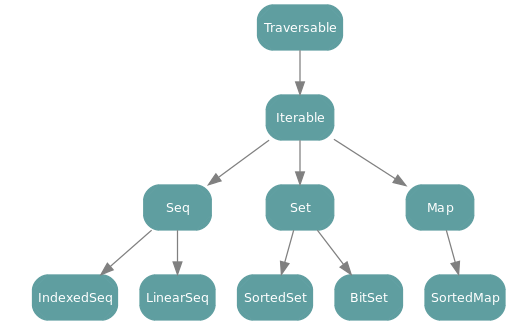
\includegraphics[width=1.0\textwidth]{../img/collection/collection-traits}
\end{Slide}
\noindent Läs mer om Scalas samlingar här: \\ 
\url{http://docs.scala-lang.org/overviews/collections/overview}
\fi

\ifkompendium\else

\begin{Slide}{Hierarki av samlingstyper i \texttt{scala.collection}}

\begin{multicols}{2}
\begin{tikzpicture}[sibling distance=6.1em,->,>=stealth', inner sep=3pt, %scale=0.5, 
  every node/.style = {shape=rectangle, draw, align=center,font=\small\ttfamily},
  class/.style = {fill=blue!20},
  trait/.style = {rounded corners, fill=red!20}]
  \node[trait] {Traversable}
    child { node[trait] {Iterable} 
      child { node[trait] {Seq} 
       }
      child { node[trait] {Set} 
      }
      child { node[trait] {Map} 
      }
    };
\end{tikzpicture}

\columnbreak
 
{\SlideFontTiny 

\code{Traversable} har metoder som är implementerade med hjälp av: \\
\code{def foreach[U](f: Elem => U): Unit}\\

\vspace{1em}\code{Iterable} har metoder som är implementerade med hjälp av: \\
\code{def iterator: Iterator[A] } 

}

\begin{itemize}\SlideFontTiny 
\item[] \code{Seq}: ordnade i sekvens
\item[] \code{Set}: unika element
\item[] \code{Map}: par av (nyckel, värde)
\end{itemize}


\end{multicols}

{\SlideFontSmall Samlingen \Emph{\texttt{Vector}} är en \code{Seq} som är en \code{Iterable} som är en \code{Traversable}.}
\end{Slide}

\begin{Slide}{Använda \texttt{iterator}}\SlideFontSmall
Med en \code{iterator} kan man \Emph{iterera} med \code{while} över alla element, men endast \Alert{en   gång}; sedan är iteratorn ''förbrukad''. (Men man kan be om en ny.)
\begin{REPL}
scala> val xs = Vector(1,2,3,4)
xs: scala.collection.immutable.Vector[Int] = Vector(1, 2, 3, 4)

scala> val it = xs.iterator
it: scala.collection.immutable.VectorIterator[Int] = non-empty iterator

scala> while (it.hasNext) print(it.next)
1234

scala> it.hasNext
res1: Boolean = false

scala> it.next
java.util.NoSuchElementException: reached iterator end
  at scala.collection.immutable.VectorIterator.next(Vector.scala:674)
\end{REPL}
\Emph{Normalt} behöver man \Alert{inte} använda \code{iterator}: det finns oftast färdiga metoder som gör det man vill, till exempel \code{foreach}, \code{map}, \code{sum}, \code{min} etc.
\end{Slide}

\begin{Slide}{Några användbara metoder på samlingar}\SlideFontTiny
\begin{tabular}{r r l}
\texttt{\Emph{Traversable}} & & \\
  & \code|xs.size| & antal elementet \\
  & \code|xs.head| & första elementet \\
  & \code|xs.last| & sista elementet \\
  & \code|xs.take(n)| & ny samling med de första n elementet \\
  & \code|xs.drop(n)| & ny samling utan de första n elementet \\
  & \code|xs.foreach(f)| & gör \code|f| på alla element, returtyp \code|Unit|\\
  & \code|xs.map(f)| & gör \code|f| på alla element, ger ny samling \\
  & \code|xs.filter(p)| & ny samling med bara de element där p är sant\\
  & \code|xs.mkString(",")| & en kommaseparerad sträng med alla element\\
    
\texttt{\Emph{Iterable}} & & \\
  & \code|xs.zip(ys)| & ny samling med par (x, y); ''zippa ihop'' xs och ys \\
  & \code|xs.zipWithIndex| & ny samling med par (x, index för x) \\
  & \code|xs.sliding(n)| & ny samling av samlingar genom glidande ''fönster''\\

\texttt{\Emph{Seq}} & & \\
  & \code|xs.length| & samma som \code|xs.size| \\
  & \code|xs :+ x| & ny samling med x sist efter xs \\
  & \code|x +: xs| & ny samling med x före xs \\
  
\end{tabular}

\pause
\vspace{0.5em}\Emph{Minnesregel} för \code{+:} och \code{:+  } \Alert{Colon on the collection side}

\pause
Prova fler samlingsmetoder ur snabbreferensen: ~~\url{http://cs.lth.se/quickref}
\end{Slide}

\begin{Slide}{Mer specifik samlingstyper i \texttt{scala.collection}}
Det finns \Alert{mer specifika} \Emph{subtyper} av \code{Seq}, \code{Set} och \code{Map}:
\\ \vspace{1em}

\begin{tikzpicture}[sibling distance=5.8em,->,>=stealth', inner sep=3pt, %scale=0.5, 
  every node/.style = {shape=rectangle, draw, align=center,font=\small\ttfamily},
  class/.style = {fill=blue!20},
  trait/.style = {rounded corners, fill=red!20}]
  \node[trait] {Traversable}
    child { node[trait] {Iterable} 
      child { node[trait, xshift=-2.4cm] {Seq} 
        child { node[trait] {IndexedSeq} }
        child { node[trait] {LinearSeq} }
       }
      child { node[trait, yshift=-0.0cm] {Set} 
        child { node[trait] {SortedSet} }
        child { node[trait] {BitSet} }
      }
      child { node[trait, xshift=1.0cm] {Map} 
        child { node[trait] {SortedMap} }
      }
    };
\end{tikzpicture}

\vspace{0.5em}
\Emph{\texttt{Vector}} är en \Alert{\texttt{IndexedSeq}} medan
\Emph{\texttt{List}} är en \Alert{\texttt{LinearSeq}}.
\end{Slide}

\begin{Slide}{Några oföränderliga och förändringsbara sekvenssamlingar}\SlideFontSmall
\begin{tabular}{r l l}
\texttt{scala.collection.\Emph{immutable}.Seq.} & & \\
 & \code|IndexedSeq.| & \\
 & & \Emph{\texttt{Vector}} \\
 & & \Emph{\texttt{Range}} \\
 & \code|LinearSeq.| & \\
 & & \Emph{\texttt{List}} \\
   & & \Emph{\texttt{Queue}} \\

\texttt{scala.collection.\Alert{mutable}.Seq.} & & \\
 & \code|IndexedSeq.| & \\
 & & \Alert{\texttt{ArrayBuffer}} \\
 & & \Alert{\texttt{StringBuilder}} \\
 & \code|LinearSeq.| & \\
 & & \Alert{\texttt{ListBuffer}} \\
   & & \Alert{\texttt{Queue}} \\
\end{tabular}

Studera samlingars egenskaper här: \href{http://docs.scala-lang.org/overviews/collections/overview}{docs.scala-lang.org/overviews/collections/overview}
\end{Slide}


\begin{Slide}{scala.collection.immutable}
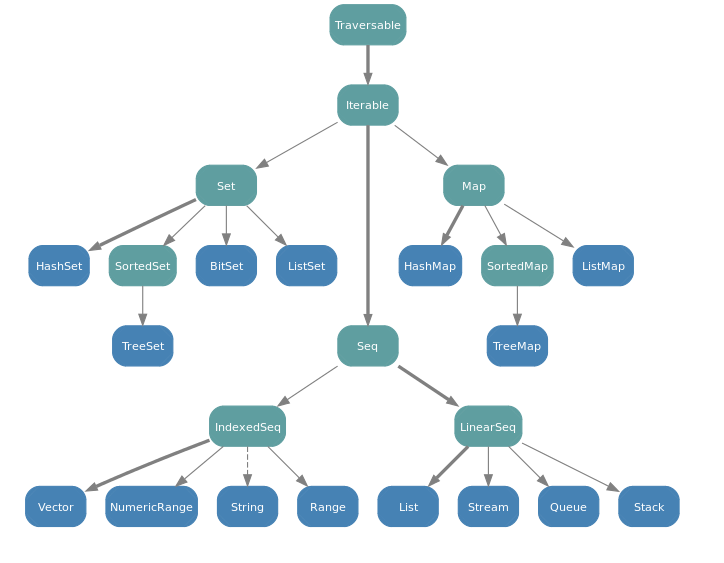
\includegraphics[width=0.82\textwidth]{../img/collection/collection-immutable}
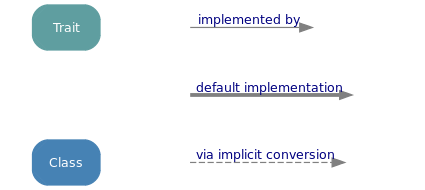
\includegraphics[width=0.33\textwidth]{../img/collection/collection-legend}
\end{Slide}


\begin{Slide}{scala.collection.mutable}
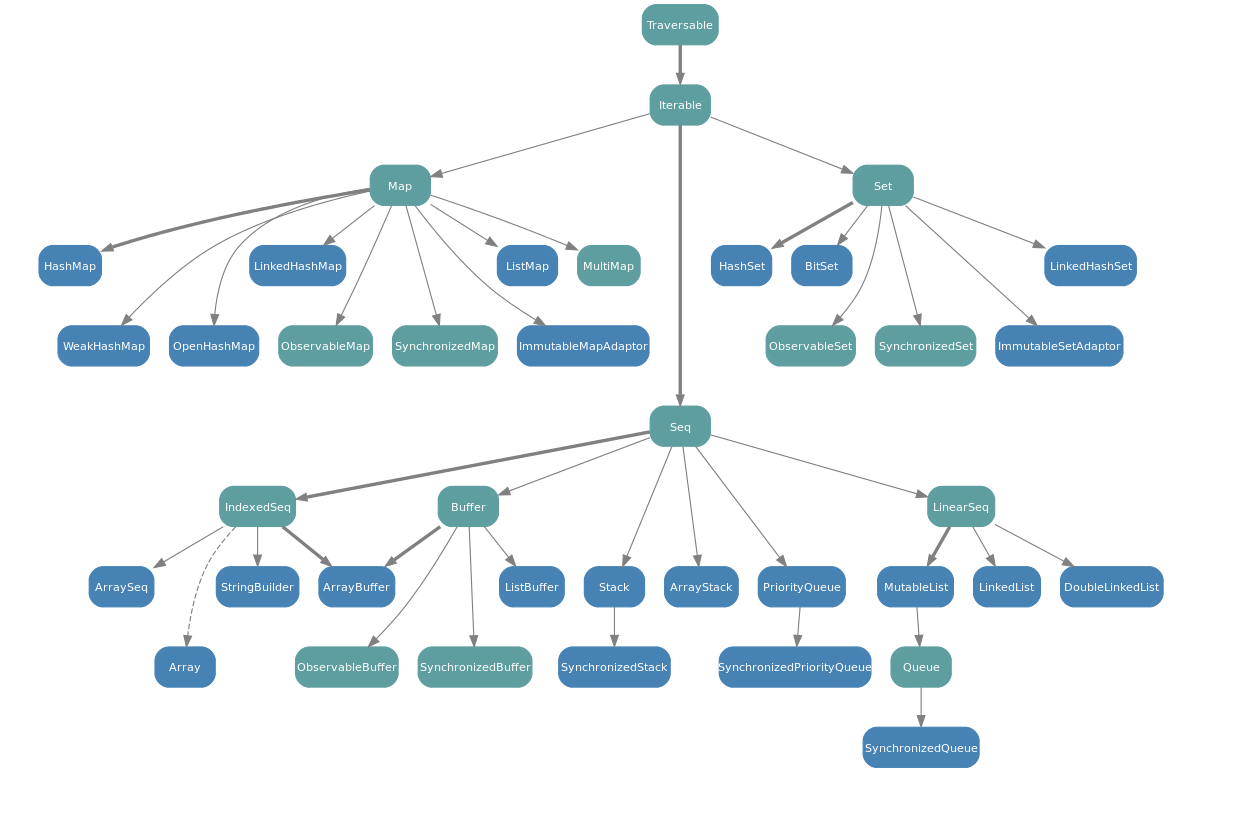
\includegraphics[width=1.05\textwidth]{../img/collection/collection-mutable}
\end{Slide}


\begin{Slide}{Strängar är implicit en \texttt{IndexedSeq[Char]}}\SlideFontSmall
Det finns en så kallad \Emph{implicit konvertering} mellan \code{String} och \code{IndexedSeq[Char]} vilket gör att \Alert{alla samlingsmetoder på \texttt{Seq} funkar även på strängar} och även flera andra smidiga strängmetoder erbjuds \Alert{utöver} de som finns i \href{http://docs.oracle.com/javase/8/docs/api/java/lang/String.html}{\code{java.lang.String}} genom klassen \href{http://www.scala-lang.org/api/current/#scala.collection.immutable.StringOps}{\code{StringOps}}.

\vspace{0.5em}
\begin{REPLnonum}
scala> "hej".  //tryck på TAB och se alla strängmetoder
\end{REPLnonum}
Detta är en stor fördel med Scala jämfört med många andra språk, som har strängar som inte kan allt som andra sekvenssamlingar kan.
\end{Slide}


\begin{Slide}{\texttt{Vector} eller \texttt{List}?}\SlideFontTiny
{\href{http://stackoverflow.com/questions/6928327/when-should-i-choose-vector-in-scala}{stackoverflow.com/questions/6928327/when-should-i-choose-vector-in-scala}}

\begin{enumerate}
\item If we only need to transform sequences by operations like map, filter, fold etc: basically it does not matter, we should program our algorithm generically and might even benefit from accepting parallel sequences. For sequential operations List is probably a bit faster. But you should benchmark it if you have to optimize.

\item If we need a lot of random access and different updates, so we should use vector, list will be prohibitively slow.

\item If we operate on lists in a classical functional way, building them by prepending and iterating by recursive decomposition: use list, vector will be slower by a factor 10-100 or more.

\item If we have an performance critical algorithm that is basically imperative and does a lot of random access on a list, something like in place quick-sort: use an imperative data structure, e.g. ArrayBuffer, locally and copy your data from and to it.
\end{enumerate}
{\href{http://stackoverflow.com/questions/20612729/how-does-scalas-vector-work}{stackoverflow.com/questions/20612729/how-does-scalas-vector-work}}\\
Mer om tids- och minneskomplexitet i fördjupningskursen och senare kurser.
\end{Slide}



\begin{Slide}{Mängd: snabb innehållstest, garanterat dubblettfri}\SlideFontSmall
En \Emph{mängd} \Eng{set} är en samling som \Alert{inte} kan innehålla \Alert{dubbletter} och som är snabb på att avgöra om ett element \Alert{finns eller inte} i mängden.

\begin{REPL}
scala> var veg = Set.empty[String]
veg: scala.collection.immutable.Set[String] = Set()

scala> veg = veg + "Gurka"
veg: scala.collection.immutable.Set[String] = Set(Gurka)

scala> veg = veg ++ Set("Broccoli", "Tomat", "Gurka")
veg: scala.collection.immutable.Set[String] = Set(Gurka, Broccoli, Tomat)

scala> veg.contains("Gurka")
res0: Boolean = true

scala> veg.apply("Gurka")   // samma som contains
res1: Boolean = true

scala> veg("Morot")
res2: Boolean = false
\end{REPL}

\end{Slide}

\begin{Slide}{Den fantastiska nyckel-värde-tabellen \texttt{Map}}\SlideFontSmall
\begin{itemize}
\item En \Emph{nyckel-värde-tabell} \Eng{key-value table} är en slags generaliserad vektor där man kan ''indexera'' med godtycklig typ. 

\item Kallas öven \href{https://sv.wikipedia.org/wiki/Hashtabell}{\Emph{hashtabell}} \Eng{hash table}, \Emph{lexikon} \Eng{dictionary} eller kort och gott \Emph{mapp} \Eng{map},

\item En hashtabell är en \Emph{mängd av par}, där varje par består av en \Emph{nyckel} och ett \Emph{värde}. 

\item Om man vet nyckeln kan man få fram värdet \Alert{snabbt}, på liknande sätt som indexering sker i en vektor om man vet heltalsindex. 

\item Denna datastruktur är \Alert{mycket användbar} och liknar en enkel databas.
\end{itemize}
\begin{REPL}
scala> val födelse = Map("C" -> 1972,  "C++" -> 1983, "C#" -> 2000, 
  "Scala" -> 2014, "Java" -> 1995, "Javascript" -> 1995, "Python" -> 1991)

födelse: scala.collection.immutable.Map[String,Int] = Map(Scala -> 2014, C# -> 2000, Python -> 1991, Javascript -> 1995, C -> 1972, C++ -> 1983, Java -> 1995)
  
scala> födelse.apply("Scala")
res0: Int = 2014

scala> födelse("Java")
res1: Int = 1995

\end{REPL}
\end{Slide}

\begin{Slide}{Speciella metoder på nyckel-värde-tabeller}
\begin{REPLnonum}
scala> val vegofärg =  Map(
               "gurka"     -> "grön", 
               "tomat"     -> "röd", 
               "aubergine" -> "lila"
            )
\end{REPLnonum}
\begin{itemize}
\item \code{xs.keySet} ger en mängd av alla nycklar
\item \code{xs.map(f)} mappar funktionen f på alla par av (key, value)
\item \code{xs.mapValues(f)} mappar funktionen map på alla värden 
\end{itemize}

\end{Slide}


\begin{Slide}{Speciella metoder på förändringsbara samlingar}\SlideFontSmall
Både \code{Set} och \code{Map} finns i \Alert{förändringsbara} varianter med extra metoder för uppdatering av innehållet ''på plats'' utan att nya samlingar skapas.
\begin{REPL}
scala> import scala.collection.mutable

scala> val ms = mutable.Set.empty[Int]
ms: scala.collection.mutable.Set[Int] = Set()

scala> ms += 42
res0: ms.type = Set(42)

scala> ms += (1, 2, 3, 1, 2, 3); ms -= 1
res1: ms.type = Set(2, 42, 3)

scala> ms.mkString("Mängd: ", ", ", s" Antal: ${ms.size}")
res2: String = Mängd: 1, 2, 42, 3 Antal: 4

scala> val ordpar = mutable.Map.empty[String, String]
scala> ordpar += ("hej" -> "svejs", "abra" -> "kadabra", "ada" -> "lovelace")
scala> println(ordpar("abra"))
kadabra
\end{REPL}
\end{Slide}

\begin{Slide}{Fler användbara samlingsmetoder}
Exempel: räkna bokstäver i ord.  \\
Undersök vad som händer i REPL:
\begin{Code}[basicstyle=\SlideFontSize{9}{13}\ttfamily]
val ord = "sex laxar i en laxask sju sjösjuka sjömän" 
val uppdelad = ord.split(' ').toVector
val ordlängd = uppdelad.map(_.length)
val ordlängMap = uppdelad.map(s => (s, s.size)).toMap
val grupperaEfterFörstaBokstav = uppdelad.groupBy(s => s(0))
val bokstäver = ord.toVector.filter(_ != ' ')
val antalX = bokstäver.count(_ == 'x')
val grupperade = bokstäver.groupBy(ch => ch)
val antal = grupperade.map(kv => (kv._1, kv._2.size))
val sorterat = antal.toVector.sortBy(_._2)
val vanligast = antal.maxBy(_._2)
\end{Code}
\end{Slide}


\begin{Slide}{Jobba med föränderlig samling lokalt; \\ returnera oföränderlig samling när du är klar}
\SlideFontSmall
Om du vill implementera en imperativ algoritm med en föränderlig samling:\\ 
Gör gärna detta \Alert{lokalt} i en \Alert{förändringsbar} samling och returnera sedan en \Emph{oföränderlig} samling, genom att köra t.ex. \code{toSet} på en mängd, eller \code{toMap} på en hashtabell, eller \code{toVector} på en \code{ArrayBuffer} eller \code{Array}.

\begin{REPL}
scala> :paste
def kastaTärningTillsAllaUtfallUtomEtt(sidor: Int = 6) = {
  val s = scala.collection.mutable.Set.empty[Int]
  var n = 0
  while (s.size < sidor - 1) {
    s += (math.random * sidor + 1).toInt
    n += 1
  }
  (n, s.toSet)
}
scala> kastaTärningTillsAllaUtfallUtomEtt()
res0: (Int, scala.collection.immutable.Set[Int]) = (13,Set(5, 1, 6, 2, 3))

\end{REPL}

\end{Slide}
\fi







%!TEX encoding = UTF-8 Unicode
%!TEX root = ../lect-week04.tex

\ifkompendium\else
\Subsection{Integrerad utvecklingsmiljö (IDE)}

\begin{Slide}{Välja IDE}\SlideFontSmall
\begin{itemize}
\item En \Emph{integrerad utvecklingsmiljö} \Eng{Integrated Development Environment, IDE} innehåller \\ editor + kompilator + debugger + en massa annat\\och gör utvecklingen enklare när man lärt sig alla finesser.

\item Läs om vad en IDE kan göra i appendix D\\(ingår i labbförberedelserna för lab \texttt{pirates}).

\pause

\item På LTH:s datorer finns två populära IDE installerade:
\begin{enumerate}\SlideFontSmall
\item \Emph{Eclipse} med plugin \Emph{ScalaIDE} förinstallerad
\begin{REPL}[numbers=none]
$ scalaide
\end{REPL}
\item \Emph{IntelliJ IDEA} (välj installera Scala-plugin när du kör första gången)  
\begin{REPL}[numbers=none]
$ idea
\end{REPL}

\end{enumerate}
Läs mer om dessa i appendix D innan du väljer vilken du vill lära dig. Där står även hur du installerar dem på din egen dator. \\Flest handledare har störst vana vid Eclipse.
\end{itemize}
\end{Slide}

\begin{Slide}{Eclipse med ScalaIDE}
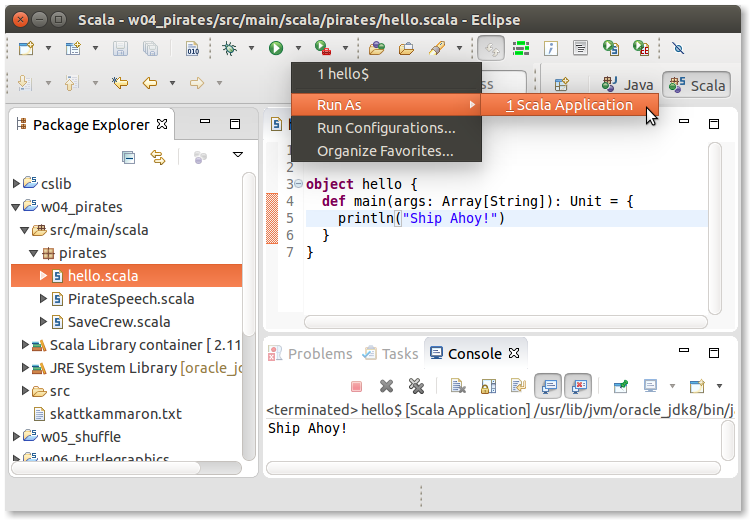
\includegraphics[width=\textwidth]{../img/eclipse/eclipse-pirates-hello.png}
\end{Slide}


\begin{Slide}{IntelliJ IDEA med Scala-plugin}
\hspace*{-0.75cm}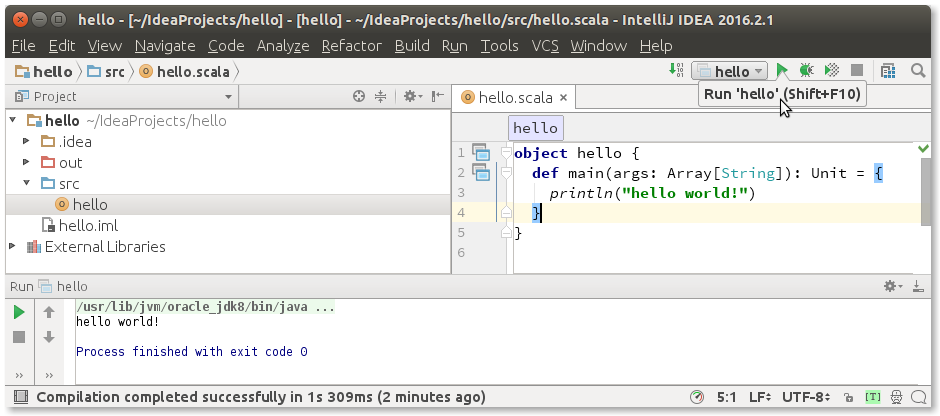
\includegraphics[width=1.15\textwidth]{../img/intellij/idea-hello.png}
\end{Slide}

\begin{Slide}{Denna veckas övning: \texttt{data}}
\begin{itemize}\SlideFontTiny
%!TEX encoding = UTF-8 Unicode
%!TEX root = ../compendium.tex

\item Kunna skapa och använda tupler, som variabelvärden, parametrar och returvärden.

\item Förstå skillnaden mellan ett objekt och en klass och kunna förklara betydelsen av begreppet instans.

\item Kunna skapa och använda attribut som medlemmar i objekt och klasser och som som klassparametrar.

\item Beskriva innebörden av och syftet med att ett attribut är privat.

\item Kunna byta ut implementationen av metoden \code{toString}.

\item Kunna skapa och använda en objektfabrik med metoden \code{apply}.

\item Kunna skapa och använda en enkel case-klass.

\item Kunna använda operatornotation och förklara relationen till punktnotation.

\item Förstå konsekvensen av uppdatering av föränderlig data i samband med multipla referenser.

\item Känna till och kunna använda några grundläggande metoder på samlingar.

\item Känna till den principiella skillnaden mellan \code{List} och \code{Vector}.

\item Kunna skapa och använda en oföränderlig mängd med klassen \code{Set}.

\item Förstå skillnaden mellan en mängd och en sekvens.

\item Kunna skapa och använda en nyckel-värde-tabell, \code{Map}.

\item Förstå likheter och skillnader mellan en \code{Map} och en \code{Vektor}.


\end{itemize}
\end{Slide}

\begin{Slide}{Denna veckas laboration: \texttt{pirates}}
\begin{itemize}\SlideFontSmall
%!TEX encoding = UTF-8 Unicode
%!TEX root = ../compendium.tex

\item Kunna använda en integrerad utvecklingsmiljö (IDE).
\item Kunna använda färdiga funktioner för att läsa till, och skriva från, textfil.
\item Kunna använda enkla case-klasser.
\item Kunna skapa och använda enkla klasser med föränderlig data.
\item Kunna använda samlingstyperna \code{Vector} och \code{Map}.
\item Kunna skapa en ny samling från en befintlig samling.
\item Förstå skillnaden mellan kompileringsfel och exekveringsfel.
\item Kunna felsöka i små program med hjälp av utskrifter.
\item Kunna felsöka i små program med hjälp av en debugger i en IDE. 


\end{itemize}
\end{Slide}

\fi







\end{document}






